\documentclass[11pt]{article}

\usepackage{graphicx}
\usepackage{hyperref}
\usepackage{natbib}
\usepackage{amsmath}

\bibliographystyle{plain}
\setlength{\textwidth}{6.5in}
\setlength{\headheight}{0in}
\setlength{\textheight}{8.0in}
\setlength{\hoffset}{0in}
\setlength{\voffset}{0in}
\setlength{\oddsidemargin}{0in}
\setlength{\evensidemargin}{0in}


\title{Computational Physics -  Problem Set 9}
  
\author{Frederik Holst Knudsen}


\begin{document}

\maketitle
Github URL: https://github.com/frederikholst/phys-ga2000
\section{Newman 8.6: The Simple Harmonic Oscillator}

PART A + B
We first rewrite the SHO as two coupled, first order differential equations. After setting $\omega=1$, we find:

\begin{equation}
    \frac{dy}{dt}=-x
    \frac{dx}{dt}=y
\end{equation}

Following Newman, we now implement the solver. Using Euler's method: 
\begin{equation}
    y^{(n+1)}=y^{(n)}+\Delta t \frac{dy}{dt}
    x^{(n+1)}=x^{(n)}+\Delta t \frac{x}{dt}
\end{equation}

See Figure \ref{SHO} where we have intial conditions of both x=1 and x=2 confirming that amplitude doesn't affect the period of oscillation. 
\begin{figure}[!htbp]
    \centering
    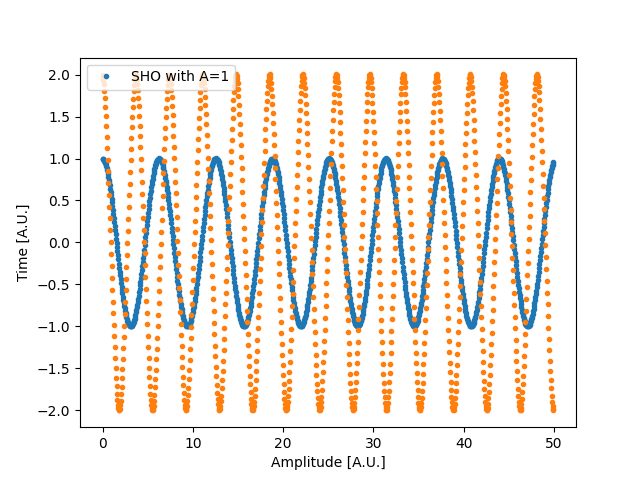
\includegraphics[width=0.6\textwidth]{SHO1.png}
    \caption{The SHO is solved using two coupled first order equation with $\frac{dx}{dt}|_{t=0}=0$ for both and $x(t=0)=1$ and $x(t=0)=2$ confirming that period is not dependent on amplitude}.
    \label{SHO}
\end{figure}

PART C
See Figure \ref{AHO} for an anharmonic oscillator  (AHO)with different amplitude and, with $\frac{d^2x}{dt^2}=-\omega^2x^3$, amplitude dependent period. 


\begin{figure}[!htbp]
    \centering
    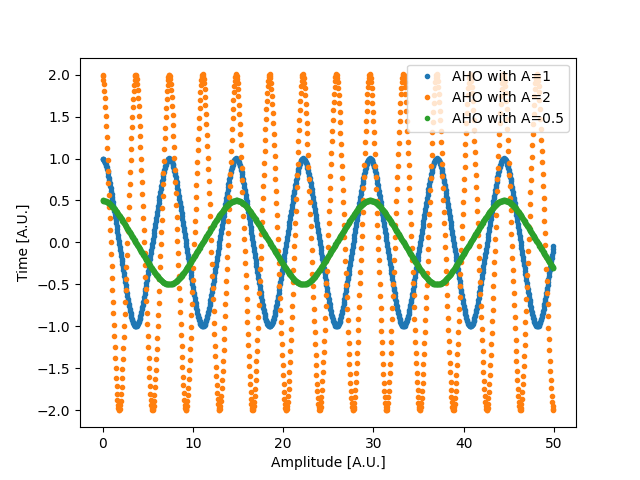
\includegraphics[width=0.6\textwidth]{AHO.png}
    \caption{AHO with A=0.5, A=1 and A=2.0 are seen with different period of oscillating as expected.}
    \label{AHO}
\end{figure}

PART D
In Figure \ref{phase} we see, as expected the ellipses in phase space of the SHO. 
\begin{figure}[!htbp]
    \centering
    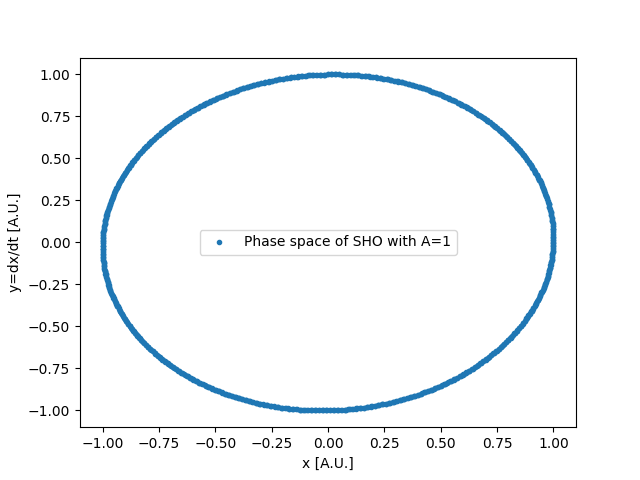
\includegraphics[width=0.7\textwidth]{phase.png}
    \caption{Ellipses in phase space with A=1 and dx/dt=0 as initial conditions.}
    \label{phase}
\end{figure}

PART E
We finally plot the phase space of van der Pol oscillator. This is readily implemented in the solver by simply updating $y=\frac{dx}{dt}$ by:

\begin{equation}
    y^{(n+1)}=y^{(n)}+\Delta t(-x+\mu(1-x^2)y)
\end{equation}

See Figure \ref{Pol} for a phase space diagram of the van der Pol oscillator. 
\begin{figure}[!htbp]
    \centering
    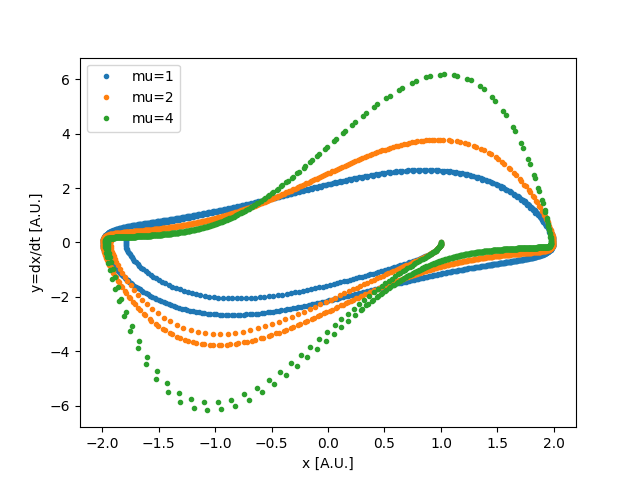
\includegraphics[width=0.7\textwidth]{Pol.png}
    \caption{Phase space portraits of van der Pol oscillator with $\mu=1$, $\mu=2$, $\mu=4$ respectively and $A=1$.}
    \label{Pol}
\end{figure}

\section{Newman 8.7}
First we show that a set of possible values of $R$, $\rho$, $C$, $m$, and $g$ maps to a one-arameter family of solutions. We rescale $t$ and $x$:

\begin{equation}
    t\rightarrow t'= \frac{t}{T}
\end{equation}
We set the characteristic length scale to be L, where the actual value is left to be determined:
\begin{equation}
    x \rightarrow x'=\frac{x}{L}
\end{equation}
Plugging into the second order differential equations given in the problem, we have for the x-direction:

\begin{equation}
    \frac{d^2x}{dt^2}=-\frac{\pi R^2 \rho C \frac{dx}{dt}\sqrt{(\frac{dx}{dt})^2+(\frac{dy}{dt})^2}}{2m}
\end{equation}

\begin{equation}
    \Rightarrow \frac{L}{T^2}\frac{d^2x'}{dt'^2}=-\frac{\pi R^2 \rho C \frac{L^2}{T^2}\frac{dx'}{dt'}\sqrt{(\frac{dx'}{dt'})^2+(\frac{dy'}{dt'})^2}}{2m}
\end{equation}

\begin{equation}
    \Rightarrow \frac{d^2x'}{dt'^2}=-\frac{\pi R^2 \rho C L\frac{dx'}{dt'}\sqrt{(\frac{dx'}{dt'})^2+(\frac{dy'}{dt})^2}}{2m}
\end{equation}

and similarly with y: 

\begin{equation}
    \frac{L}{T^2}\frac{d^2y'}{dt'^2}=-g-\frac{\pi R^2 \rho C \frac{L^2}{T^2}\frac{dy'}{dt'}\sqrt{(\frac{dx'}{dt'})^2+(\frac{dy'}{dt'})^2}}{2m}
\end{equation}


\begin{equation}
    \Rightarrow \frac{d^2y'}{dt'^2}=-g\frac{T^2}{L}-\frac{\pi R^2 \rho C L\frac{dy'}{dt'}\sqrt{(\frac{dx'}{dt'})^2+(\frac{dy'}{dt'})^2}}{2m}
\end{equation}

To make the equations dimonsionless and controlled by a single parameter, we choose $L$ so that it removes the first term of the equation in y:
\begin{equation}
    L\equiv \frac{1}{2}gT^2
\end{equation}


\begin{equation}
    \Rightarrow \frac{d^2y'}{dt'^2}=-2-\lambda \frac{dy'}{dt'}\sqrt{(\frac{dx'}{dt'})^2+(\frac{dy'}{dt'})^2}
\end{equation}

Similarly for x:

\begin{equation}
    \Rightarrow \frac{d^2x'}{dt'^2}=-\lambda\frac{dx'}{dt'}\sqrt{(\frac{dx'}{dt'})^2+(\frac{dy'}{dt'})^2}
\end{equation}.

And we have a dimensionless equation with one free paramter, $\lambda$.


PART A
First we compute the drag force in the x-direction:

Since the x-component of the drag force is found by: 
\begin{equation}
    \overrightarrow{F}_ {Drag}=-|F_{Drag}| \cdot  \widehat{v} 
\end{equation}
where:
\begin{equation}
    \widehat{v}=\frac{(v_x,v_y)}{\sqrt{(v_x^2+v_y^2)}}
\end{equation}.
From Newton's second law, we then have for the x-direction:
\begin{equation}
    F_x=ma_x=m*\frac{d^2x}{dt^2}=\frac{\pi R^2 \rho C v_xv}{2}
\end{equation}

Solving for $\frac{d^2x}{dt^2}$ we find: 
\begin{equation}
    \frac{d^2x}{dt^2}=-\frac{\pi R^2 \rho C v_xv}{2m}
\end{equation}

Similarly for y, except for the gravity acting in this direction:
\begin{equation}
    F_x=ma_y=m*\frac{d^2y}{dt^2}=-gm-\frac{\pi R^2 \rho C v_yv}{2}
\end{equation}

Solving for $\frac{d^2y}{dt^2}$ we find: 
\begin{equation}
    \frac{d^2y}{dt^2}=-g-\frac{\pi R^2 \rho C v_yv}{2m}
\end{equation}

PART B
See Figure \ref{cannon} for a trajectory of a cannonball with $v_0=100 \frac{m}{s}$ and fired at an angle of 30 degrees. We see, as expected, that the velocities in both directions gets damped over time, and that the gravitational force in the downward direction dominates in the end. 
\begin{figure}[!htbp]
    \centering
    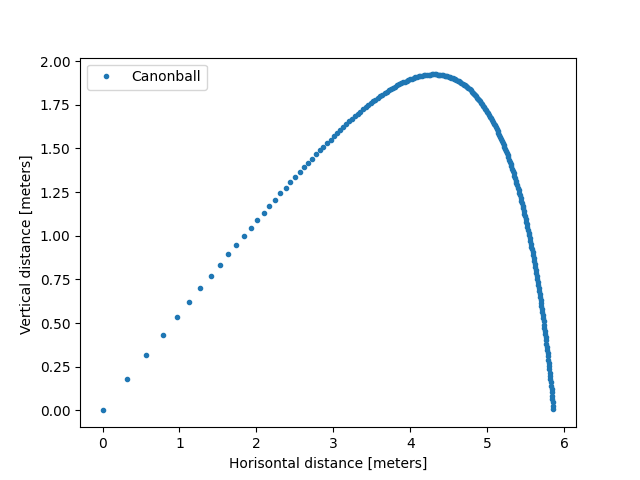
\includegraphics[width=0.7\textwidth]{cannon.png}
    \caption{The canonball is fired in a constant gravitational field fired with $v_0=100 \frac{m}{s}$ at 30 degrees and is damped due to air resistance.}
    \label{cannon}
\end{figure}

PART C
See Figure \ref{mass} for a graph of the distance traveled as a function of mass. We see a linear increase in distance traveled. The reason is that the damping factor goes as $\approx\frac{1}{m}$, but the gravitational force doesn't, so the ball is relatively less damped and thus travel further. 

\begin{figure}[!htbp]
    \centering
    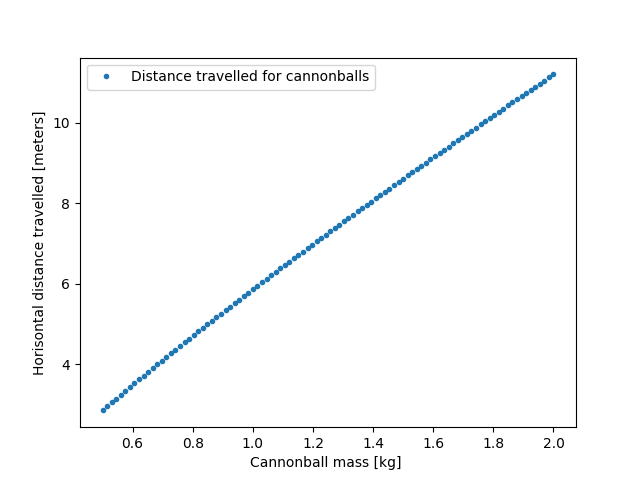
\includegraphics[width=0.7\textwidth]{mass.png}
    \caption{Cannonballs plotted with distance travelled against mass. We see a linear dependence. }
    \label{mass}
\end{figure}


\end{document}

\begin{figure}[!htbp]
    \centering
    \includegraphics[width=0.7\textwidth]{.png}
    \caption{}
    \label{v}
\end{figure}
